\chapter{Топология в $\mathbb{R}^n$}

\section{Пространство $\mathbb{R}^n$}

\begin{definition}
    
Множество, обозначаемое через $\mathbb{R}^n$, определятся следующим образом
\[
 \mathbb{R}^n: = \underbrace{\mathbb{R} \times \cdots \times  \mathbb{R}}_n.
\]

При этом, для любых $\alpha,\beta \in \mathbb{R}$, и $\mathbf{x}=(x_1,\ldots, x_n), \mathbf{y} = (y_1,\ldots, y_n) \in \mathbb{R}^n$;
\[
 \alpha \mathbf{x} + \beta \mathbf{y}: = (\alpha x_1 + \beta y_1, \ldots, \alpha x_n + \beta y_n). 
\]
\end{definition}


Таким образом, $\mathbb{R}^n$ -- это линейное пространство или векторное пространство над полем $\mathbb{R}$. Из курса линейной алгебры хорошо известно, что любое конечномерное пространство размерности $n$ изоморфно векторному пространству $\mathbb{R}^n$. Этот изоморфизм, фактически, задаётся введением координат.

Когда мы будем говорить об $\mathbb{R}^n$ как о векторном пространстве, то каждый набор будем записывать как вектор, \ie в виде $\mathbf{x} = \begin{pmatrix} x_1 \\ \vdots \\ x_n \end{pmatrix} = (x_1,\ldots, x_n)^\top.$ Нулевой вектор пространства $\mathbb{R}^n$ мы будем обозначать так $\m{0}_n$, таким образом $\m{0}_n = (0,\ldots, 0)^\top.$

Возьмём $\mathbf{x} = (x_1,\ldots, x_n)^\top \in \mathbb{R}^n$, тогда ясно, что 
\[
\begin{pmatrix}
    x_1 \\ \vdots \\x_n 
\end{pmatrix} = x_1 \begin{pmatrix}
    1 \\ \vdots \\ 0
\end{pmatrix} + \cdots + x_n \begin{pmatrix}
    0 \\ \vdots \\1
\end{pmatrix}
\]

Множество $\mathbb{e} = \{\mathbf{e}_1, \ldots, \mathbf{e}_n\}$, где $\mathbf{e}_1 = (1,0, \ldots, 0)^\top, \ldots, \mathbf{e}_n = (0,0,\ldots, 1)^\top$, называется \textit{базисом} пространства $\mathbb{R}^n.$

\subsection{Отображения в $\mathbb{R}^n$}

\begin{definition}
 \textit{Линейное отображение} $f:\mathbb{R}^n \to \mathbb{R}^m$ -- это такое отображение, что $f(\alpha \m{x} +\beta \m{y} ) = \alpha f(\m{x}) +\beta f(\m{y})$, где $\m{x,y} \in \mathbb{R}^n$, $\alpha, \beta \in \mathbb{R}.$     
\end{definition}

\begin{mydangerr}{\bf !}
    В частности это значит, что $f(\m{0_n}) = \m{0_m}.$
\end{mydangerr}

В таком случае, линейное отображение $f:\mathbb{R}^n \to \mathbb{R}^m$ достаточно задать на базисных векторах;

\[
 \begin{pmatrix}
     1 \\ \vdots \\ 0
 \end{pmatrix} \mapsto \begin{pmatrix}
     a_{11} \\ \vdots \\ a_{m1}
 \end{pmatrix}, \ldots, \begin{pmatrix}
     0 \\ \vdots \\ 1
 \end{pmatrix} \mapsto \begin{pmatrix}
     a_{1n} \\ \vdots \\ a_{mn}
 \end{pmatrix}.
\]

Возьмём теперь произвольный вектор $\m{x} \in \m{V}$, и пусть $\mathbb{e} =  \{\m{e}_1,\ldots, \m{e}_n\}$ -- базис в $\m{V}$, тогда его можно расписать следующим образом
\[
 \m{x} = x_1 \m{e}_1 + \cdots + x_n \m{e}_n.
\]

Поэтому, если $f$ -- линейное отображение, то
\begin{eqnarray*}
    f(\m{x}) &=& f(x_1 \m{e}_1 + \cdots + x_n \m{e}_n) \\
    &=& x_1 f(\m{e}_1) + \cdots + x_n f(\m{e}_n) \\
    &=& x_1 \begin{pmatrix}
     a_{11} \\ \vdots \\ a_{m1}
 \end{pmatrix} + \cdots + x_n \begin{pmatrix}
     a_{1n} \\ \vdots \\ a_{mn}
 \end{pmatrix},
\end{eqnarray*}
поэтому естественно записать в матричном виде это отображение следующим образом
\[
 f: \begin{pmatrix}
     x_1 \\ 
     \vdots \\
     x_n
 \end{pmatrix} \mapsto \begin{pmatrix}
     a_{11} x_1 + \cdots + a_{1n}x_n \\
     \vdots \\
     a_{m1}x_1 + \cdots + a_{mn}x_n.
 \end{pmatrix}
\]
и мы можем тогда положить
\[
 A\cdot \m{x} = \begin{pmatrix}
    a_{11} & \ldots & a_{1n} \\
    \vdots & \ddots & \vdots \\
    a_{m1} & \ldots & a_{mn}
\end{pmatrix} \cdot \begin{pmatrix}
     x_1 \\ 
     \vdots \\
     x_n
 \end{pmatrix} : = \begin{pmatrix}
     a_{11} x_1 + \cdots + a_{1n}x_n \\
     \vdots \\
     a_{m1}x_1 + \cdots + a_{mn}x_n.
 \end{pmatrix}
 \]

\begin{figure}[h!]
    \centering
    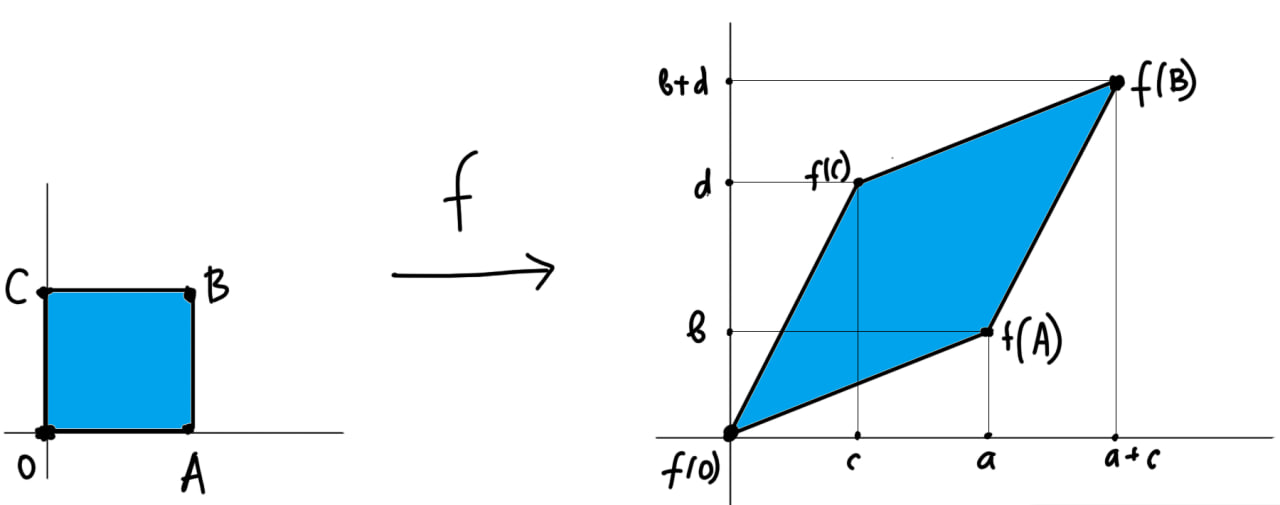
\includegraphics[scale = 0.5]{images/linear_map.jpg}
    \caption{Линейное отображение $f:\mathbb{R}^2 \to \mathbb{R}^2$, которое задаётся матрицей $A = \begin{pmatrix}
        a & c \\
        b & d
    \end{pmatrix}$. Её первый столбец это координаты образа первого базисного вектора $\m{e}_1 = (1,0)^\top$ (на рисунке слева это направленный отрезок $OA$), а её второй столбец это координаты образа второго базисного вектора $\m{e}_2 = (0,1)^\top$ (на рисунке слева это направленный отрезок $OC$).}
    \label{linear_map}
\end{figure}

Таким образом имеет место следующий результат

 \begin{theorem}\label{linear_map=matix}
Пусть $f: \mathbb{R}^n \to \mathbb{R}^m$ -- линейное отображение. Тогда существует единственная матрица $A \in \mathrm{Mat}_{m\times n}(\mathbb{R})$, такая что 
    \[
     f(\m{v}) = A\cdot \m{v}, \qquad \mbox{для всех $\m{v} \in \m{V}$}.
    \]

Более того, эта матрица имеет вид $A = \begin{pmatrix}
    f(\m{e}_1) & \ldots & f(\m{e}_n)
\end{pmatrix}$, где $\{\m{e}_1,\ldots, \m{e}_n\}$ -- какой-то базис в $\mathbb{R}^n$.
\end{theorem}


\begin{mydangerr}{\bf !}
Мы получили, что любое линейное отображение $f: \mathbb{R}^n \to \mathbb{R}^m$ кодируется матрицей, при этом её первый столбец это образ первого базисного вектора, второй столбец это образ второго базисного и.т.д.
\end{mydangerr}



\subsection{Композиция отображений и его матричное представление}


Теперь мы приступим к общему случаю, но сначала введём полезные для дальнейшего обозначения и соглашения

Пусть дана матрица $A\in \mathrm{Mat}_{n\times m}(\mathbb{R})$, 
\[
A = \begin{pmatrix}
    a_{11} & a_{12} & \ldots & a_{1n} \\
    a_{21} & a_{22} & \ldots & a_{2n} \\
    \vdots & \vdots & \ddots & \vdots \\
    a_{m1} & a_{m2} & \ldots & a_{mn} \\
\end{pmatrix}
\]
обозначим через $\m{r}_i(A):= \begin{pmatrix}
    a_{i1} & a_{i2} & \ldots & a_{in}
\end{pmatrix}$ -- её $i$-ую строку, а через $\m{c}_j(A) : = \begin{pmatrix}
    a_{1j}\\a_{2j}\\\vdots \\a_{mj}
\end{pmatrix}$ -- её $j$-ый столбец.

Тогда саму матрицу $A$ можно записать следующим образом
\[
A = \begin{pmatrix}
    a_{11} & a_{12} & \ldots & a_{1n} \\
    a_{21} & a_{22} & \ldots & a_{2n} \\
    \vdots & \vdots & \ddots & \vdots \\
    a_{m1} & a_{m2} & \ldots & a_{mn} \\
\end{pmatrix} = \begin{pmatrix}
    \m{r}_1(A) \\
    \m{r}_2(A) \\
    \vdots \\
    \m{r}_m(A)
\end{pmatrix} = \begin{pmatrix}
    \m{c}_1(A) & \m{c}_2(A) & \ldots & \m{c}_n(A)
\end{pmatrix}.
\]

Итак, пусть у нас есть три конечномерных векторных пространства $\mathbb{R}^n, \mathbb{R}^k, \mathbb{R}^m$ и два линейных отображения $g: \mathbb{R}^n \to \mathbb{R}^k$, $f:\mathbb{R}^k \to \mathbb{R}^m$. Это проще записать следующим образом
\[
 \xymatrix{
 \mathbb{R}^n \ar@{->}[r]^{g} \ar@{->}[rd]_{f\circ g} & \mathbb{R}^k \ar@{->}[d]^f \\
 & \mathbb{R}^m
 }
\]

Возьмём произвольный вектор $\m{x} \in \mathbb{R}^n$, пусть $\m{x} = x_1 \m{e}_1 + \cdots + x_n \m{e}_n$, тогда, получаем
\begin{eqnarray*}
    g(\m{x}) &=& g(x_1 \m{e}_1 + \cdots + x_n \m{e}_n) \\
    &=& x_1 g(\m{e}_1) + \cdots + x_n g(\m{e}_n) \\
    &=& x_1 \begin{pmatrix}
     b_{11} \\ \vdots \\ b_{m1}
 \end{pmatrix} + \cdots + x_n \begin{pmatrix}
     b_{1n} \\ \vdots \\ b_{mn}
 \end{pmatrix} \\
 &=& x_1 \m{c}_1(B) + \cdots + x_n \m{c}_n(B).
\end{eqnarray*}

Далее, имеем
\begin{eqnarray*}
    f(g(\m{x})) &=& f(x_1 \m{c}_1(B) + \cdots + x_n \m{c}_n(B)) \\
    &=& x_1 f(\m{c}_1(B)) + \cdots + x_n f(\m{c}_n(B)) \\
    &=& x_1 A\m{c}_1(B) + \cdots + x_n A\m{c}_n(B)
\end{eqnarray*}

Таким образом, мы получаем, что композиция отображений $f\circ g$ задаётся матрицей $M$, которая находится следующим образом
\[
 M: = \begin{pmatrix}
     A\m{c}_1(B) & \ldots & A\m{c}_n(B)
 \end{pmatrix}
\]

\begin{definition}
  Такую матрицу называют произвдением матриц $A$ и $B$ и обозначают её так $AB$.
\end{definition}

Но понятно, что одними только линейными всё не ограничивается. Ведь вовсе не обязательно, что образ прямой будет всегда прямая при любом её отображении.

Однако же, это не означает, что линейную алгебру не надо изучать. Как раз наоборот, в сущности, анализ изучает любые подобное отображения с помощью линейной алгебры; локально они устроены как раз таки линейно (см. Рис.\ref{deff+linear}).

\begin{figure}[h!]
    \centering
    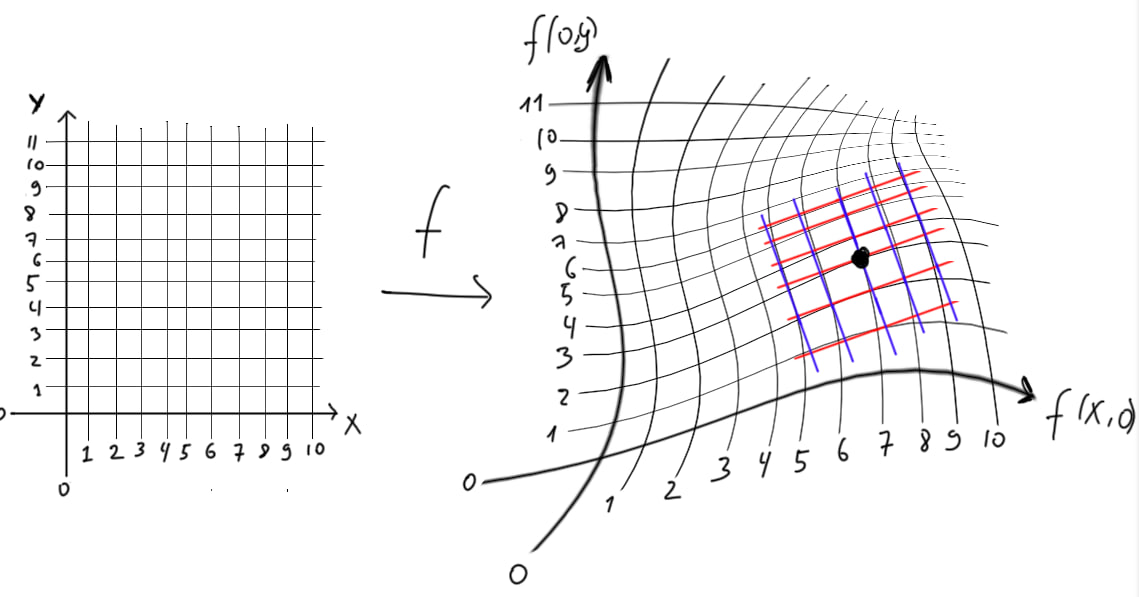
\includegraphics[scale = 0.7]{images/deff+linear.jpg}
    \caption{Пример нелинейного отображения. Однако в близи выделенной точки, это трудное отображение очень похоже на линейное.}
    \label{deff+linear}
\end{figure}


\begin{mydangerr}{\bf !}
 Поэтому мы будем изучать такие отображения которые похожи на линейные. Для того чтобы нам более чётко сформулировать нашу цель нам нужно ввести некоторые важные понятия.    
\end{mydangerr}



\section{Нормированные пространства и топология}

Напомним, что когда говорим о векторных пространствах, мы всегда имеем в виду векторные пространства (конечной или бесконечной размерности) над полем действительных чисел или над полем комплексных чисел. 

\begin{definition}
    \textit{Норма} в векторном пространстве $\m{V}$ есть отображение\footnote{обычно записываемое в виде $\m{v} \mapsto \| \m{v}\|$, причём, если потребуется, знак $ \| \cdot \|$ сопровождается индексами.} $\|\cdot\|: \m{V} \to \mathbb{R}_{\ge 0}$, обладающее следующими свойствами:
    \begin{enumerate}
        \item если $\| \m{v}\| = 0$, то $\m{V} = \m{0_V}$ -- нулевой вектор.
        \item $\|\lambda \m{v} \| = |\lambda| \cdot \| \m{v}\|$ для любого $\m{v} \in \m{V}$, $\lambda \in \mathbb{R}$.
        \item $\| \m{v+u} \| \le \|\m{v}\| + \|\m{u}\|$ для любых $\m{v,u \in V}$ (\textit{неравенство треугольника}).
    \end{enumerate}
В таком случае, если на пространстве $\m{V}$ задана норма $\|\cdot\|$, то пару $(\m{V}, \|\cdot\|)$ называют \textit{нормированным пространством.}
\end{definition}


%Из определения сразу вытекает следующее:
%%\begin{proposition}
  %   Если $x \mapsto ||x||$ -- норма в векторном пространстве $E$, то $d(x,y):=||x-y||$ -- метрика в $E$, обладающая тем свойством, что $d(x+z, y+z) = d(x,y)$, $d(\lambda x, \lambda y) = |\lambda| d(x,y)$ для любого $\lambda \in \mathbb{R}.$
%\end{proposition}


\begin{definition}
    Пусть $(\m{V}, \|?\|)$ нормированное пространство, для фиксированного вектора $\m{a} \in \m{V}$ и числа $r >0$.
    \begin{enumerate}
    \item Множество
    \[
     \mathsf{B}(\m{a}, r): = \{ \m{v}\in \m{V}\, :\, \| \m{a -v} \| < r \}
    \]
    называется \textit{открытым шаром с центром в точке $\m{a}$ и радиусом $r$.} 
    \item Множество
    \[
     \overline{\mathsf{B}}(\m{a}, r): = \{ \m{v}\in \m{V}\, :\, \| \m{a -v} \| \le r \}
    \]
    называется \textit{замкнутым шаром с центром в точке $\m{a}$ и радиусом $r$.}
    \item Множество
    \[
     \mathsf{S}(\m{a}, r): = \{ \m{v}\in \m{V}\, :\, \| \m{a -v} \| = r \}
    \]
    называется \textit{сферой с центром в точке $\m{a}$ и радиусом $r$.} 
    \end{enumerate}
        
\end{definition}


По анологии с тем как была введена топология на прямой, мы подобным образом топологию в $\mathbb{R}^n$ и вообще в любом нормированном пространстве.

\begin{definition}
    Пусть $(\m{V}, \|?\|)$ -- нормированное пространство, множество $\mathscr{U} \subseteq \m{V}$ называется \textit{открытым} если для любой точки $\m{a} \in \mathscr{U}$ существует такое число $\varepsilon>0$, что $\mathsf{B}(\m{a}, \varepsilon) \subseteq \mathscr{U}$.  Множество $F \subseteq \m{V}$ называется \textit{замкнутым} если существует такое открытое $\mathscr{U} \subseteq \m{V}$, что $F = \m{V}\setminus \mathscr{U}.$
\end{definition}

\begin{lemma}\label{open_ball=open}
Любой открытый шар в нормированном пространстве $(\m{V}, \|\cdot\|)$ является открытым множеством.
\end{lemma}
\begin{proof}
 Пусть $\mathsf{B}(\m{a},r)$ -- открытый шар, пусть $\m{v} \in \mathsf{B}(\m{a},r)$, $\m{v} \ne \m{a}$. Тогда по определению $\|\m{v-a}\| < r$. Рассмотрим теперь открытый шар $\mathsf{B}(\m{v},\delta)$, где $0 < \delta < r- \|\m{v}- \m{a}\|.$ Покажем, что $\mathsf{B}(\m{v},\delta ) \subseteq \mathsf{B}(\m{a}, r)$, это и докажет лемму.

Пусть $\m{w} \in \mathsf{B}(\m{a},\delta)$ при этом потребуем чтобы $\| \m{v} - \m{w} \|<\delta < r - \|\m{a} - \m{v}\| $, тогда по неравенству треугольника
    \[
      \|\m{a-w}\| \le \|\m{a-v}\| + \|\m{v-w}\| < \|\m{a-v}\| + r - \|\m{a-v}\| = r, 
    \]
    \ie $\m{w} \in \mathsf{B}(\m{a},r)$, что и доказывает включение $\mathsf{B}(\m{v},\delta ) \subseteq \mathsf{B}(\m{a}, r)$, так как вектор $\m{v}$ был выбран произвольно. 
\end{proof}

\begin{lemma}\label{union_and_cap_of_open}
    Объединение любого семейства открытых множеств открыто и пересечение конечного числа открытых множеств открыто. 
\end{lemma}
\begin{proof}\
 
(1) Пусть $\mathscr{U} = \cup_{\alpha \in A}\mathscr{U}_\alpha$ и пусть $x \in \mathscr{U}$, тогда для какого-то $\alpha \in A$, $x \in \mathscr{U}_a$. Так как $\mathscr{U}_\alpha$ -- открыто, то найдётся такой $r >0$, что $B(x, r ) \subseteq \mathscr{U}_\alpha \subseteq \cup_{\alpha \in A}\mathscr{U}_\alpha$, что и доказывает открытость $\mathscr{U}.$

(2) Достаточно доказать, что множество двух открытых множеств $\mathscr{U}_1, \mathscr{U}_2$ открыто, а затем провести индукцию. Если $x \in \mathscr{U}_1 \cap \mathscr{U}_2$, то найдутся такие $r_1, r_2 >0$, что $B(x, r_1) \subseteq \mathscr{U}_1$, $B(x, r_2) \subseteq \mathscr{U}_2$. Очевидно, что $B(x, r) \subseteq \mathscr{U}_1 \cap \mathscr{U}_2$, где $r:= \min(r_1, r_2)$, что и доказывает открытость пересечения.
\end{proof}

\begin{definition}
    Пусть $A$ -- непустое множество в нормированном пространстве $\m{V}$. \textit{Открытой окрестностью} множества $A$ называется любое открытое множество $\mathscr{U}(A)$, содержащее $A$. В случае, когда $A = \{x\}$, мы говорим об окрестности $\mathscr{U}(x)$ точки $x$ (а не множества $\{x\}).$
\end{definition}

\begin{mydanger}{\bf{!}}
 Очевидно, что $\mathscr{U}(x)$ можно отождествить с подходящим открытым шаром $\mathsf{B}(x,r)$, поэтому иногда мы не будем делать разницу между открытым шаром с центром в точке $x$ и открытым множеством, содержащим эту же точку $x.$    
\end{mydanger}

\section{Замкнутые множества, точки прикосновения}

\begin{definition}
    \textit{Замкнутое множество} в нормированном пространстве $\m{V}$ есть дополнение открытого множества. 
\end{definition}

Пустое множество замкнуто, замкнуто и всё пространство $\mathbb{R}^n$.


\begin{definition}\label{limit_point_in_metric}
  Пусть $\m{V}$ -- нормированное пространство, и пусть $A \subseteq \m{V}$. \textit{Точка прикосновения} множества $A$ -- такая точка $x \in \m{V}$, каждая окрестность которой имеет с $A$ непустое пересечение. Множество всех точек прикосновения называется \textit{замыканием} множества $A$ и обозначается символом $\overline{A}.$
\end{definition}


\begin{lemma}\label{closure_in_metric}
    Множество $F$ в нормированном пространстве замкнуто, если и только если все его точки это точки прикосновения, \textit{т.е.,} $F = \overline{F}.$ 
\end{lemma}
\begin{proof}
(1) Пусть $F$ -- замкнуто, тогда найдётся какое-то открытое $\mathscr{U} \subseteq \m{V}$, такое, что $F  = \m{V} \setminus \mathscr{U}$. Пусть $x \notin F$, тогда $x \in \mathscr{U}$, и тогда найдётся окрестность $\mathscr{W}(x)$ такая, что $\mathscr{W}(x) \subseteq \mathscr{U}$, потому что $\mathscr{U}$ -- открыто, \textit{т.е.,} $\mathscr{W}(x) \cap F = \varnothing.$ Таким образом, получили, что если $F$ -- замкнуто, то никакая точка $x \notin F$ не может быть точкой прикосновения для $F$, \textit{т.е.,} $F = \overline{F}.$ 

(2) Пусть $F = \overline{F}$, тогда для любой точки $x \notin F$, можно всегда найти окрестность $\mathscr{W}(x)$ такую, что $\mathscr{W}(x) \cap F = \varnothing$. Пусть $\mathscr{U}:= \cup_{x \m{V} \setminus F} \mathscr{W}(x)$, тогда, $\mathscr{U}$ -- открыто в $\m{V}$ и $F = \m{V} \setminus \mathscr{U}.$

\end{proof}








\section{Подпространства нормированного пространства}

Пусть $F \subseteq \mathbf{V}$ -- непустое подмножество нормированного пространства $\mathbf{V}$, тогда $F \times F \subseteq \mathbf{V} \times \mathbf{V}$ -- непустое подмножество, тогда мы имеем следующую коммутативную диаграмму

\[
  \begin{tikzcd}
    F \times F \arrow[hook]{d}[left]{\mathrm{in}} \arrow{dr}{\|\cdot\|_{F \times F}} &  \\
    \mathbf{V} \times \mathbf{V} \arrow{r}[below]{\|\cdot\|} & \mathbb{R}
  \end{tikzcd}
\]
\ie, \textit{сужая} норму $\|\cdot\|$ на $F$, мы получаем нормированное пространство $(F,\|\cdot\|_{F})$, которое мы будем для простоты обозначать $(F, \|\cdot\|_F)$.

\begin{definition}
    Нормированное пространство, определённое таким образом, называется \textit{подпространством} $F$ нормированного пространства $\mathbf{V}$.
\end{definition}

\begin{figure}[h!]
    \centering
    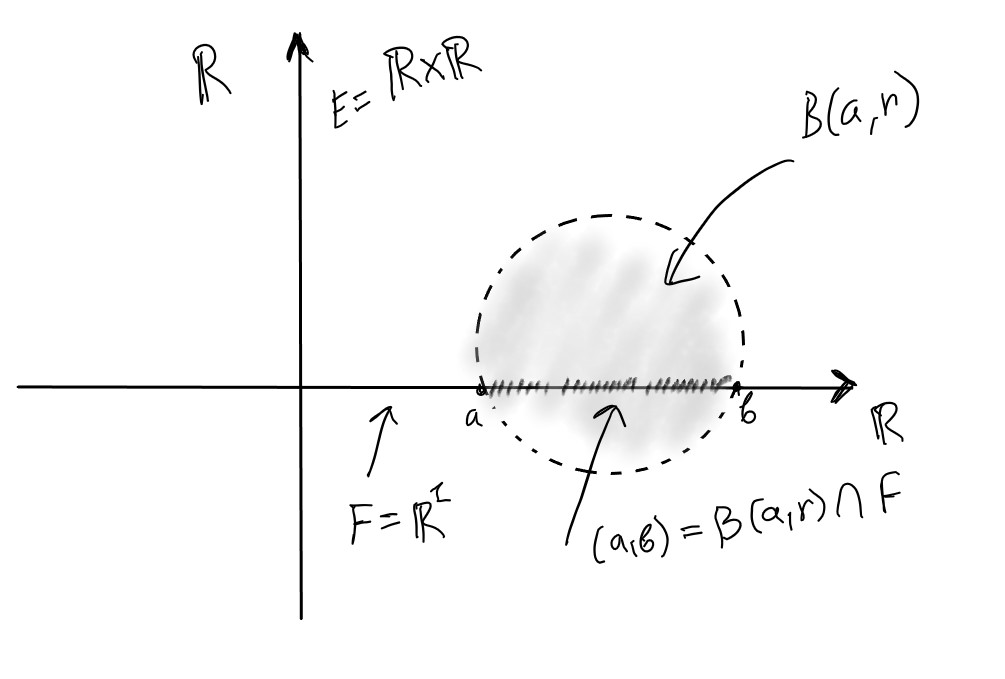
\includegraphics[scale = 0.4]{images/open_in_F.jpg}
    \caption{Пусть $\mathbf{V} = \mathbb{R} \times \mathbb{R}$ -- обыкновенная плоскость с евклидовой нормой $\|\m{x}\| = \sqrt{x_1^2 + x_2^2}$, и пусть $F = \mathbb{R}$, которую мы можем понимать как множество вида $\{(x,0), x\in \mathbb{R}\}$. На рисунке $F$ отождествлена с осью $Ox$. Тогда, сужая норму на $F$, мы получаем $\|x\|_F = |x|$. Более того, ясно, что любой интервал $(a,b)$ можно получить, пересекая открытый шар с $F.$}
    \label{fig:enter-label}
\end{figure}


\begin{proposition}\label{open_in_subset}
    Для того чтобы множество $S \subseteq F$ было открыто в подпространстве $F$, необходимо и достаточно, чтобы существовало такое множество $\mathscr{U}$, открытое в $\mathbf{V}$, что $S = \mathscr{U} \cap F.$
\end{proposition}

\begin{proof}
    Прежде всего, поймём, что есть открытый шар в $F$. Пусть $a \in F$, и рассмотрим открытый шар $B(a,r) \subseteq \mathbf{V}$, тогда получаем
    \begin{eqnarray*}
        F \cap B(a,r) &:=& \{x \in \mathbf{V} \cap F\, :\, \|x-a\|<r\} \\
        &=&\{x\in F\, :\, \|x-a\|<r\} \\
        &=& \{x \in F\, :\, \|x-a\|_F<r\},
    \end{eqnarray*}
    \ie $F \cap B(a,r)$ -- это \textbf{открытый шар в $F$ с центром в точке $a$ радиуса $r.$}

\begin{mydanger}{\bf{!}}
    Обратим внимание, что если $F = \mathbb{R}_{\ge 0} \subseteq \mathbb{R} = \mathbf{V}$, $\|x\| = |x|$, то, например, $[0,1)$ -- открытый шар в $F = \mathbb{R}_{\ge 0}$, так как $[0,1) = (-1,1) \cap \mathbb{R}_{\ge 0}$. Hо! В $\mathbb{R}$, $[0,1)$ и не открыт и не замкнут!
\end{mydanger}

(1) Пусть $\mathscr{U}$ -- открытое множество в $\mathbf{V}$, и пусть $x \in \mathscr{U} \cap F$. Так как $\mathscr{U}$ -- открытое в $\mathbf{V}$, то найдётся шар $B(x,r) \subseteq \mathbf{V}$ такой, что $B(x,r) \subseteq \mathscr{U}$. Тогда $F \cap B(x,r) \subseteq F \cup \mathscr{U}$. Но мы уже поняли, что $B(x,r) \cap F$ -- открытый шар в $F$, но тогда включение $F \cap B(x,r) \subseteq F \cup \mathscr{U}$ и означает, что $\mathscr{U} \cap F$ открыто в $F$, ибо $x$ -- произвольная точка в $\mathscr{U} \cap F.$

(2) Пусть $S$ открыто в $F$, это значит, что для любой точки $x \in S$ можно найти открытый шар $B(x, r(x)) \subseteq \mathbf{V}$ такой, что $F \cap B(x,r(x)) \subseteq S$ (т.к., $F \cap B(x,r(x))$ -- это открытый шар в $F$).

Тогда 
\[
 S = \bigcup_{x \in S} F \cap B(x, r(x)) = F \cap \mathscr{U},
\]
где $\mathscr{U} = \cup_{x\in S} B(x, r(x)) \subseteq \mathbf{V}$, тогда $\mathscr{U}$ открыто в $\mathbf{V}$ как объединение открытых шаров.
\end{proof}





\section{Сходимость в $\mathbb{R}^n$}

Для доказательства обобщённой теоремы Больцано--Вейерштрасса нам понадобится следующее ключевое неравенство:

\begin{lemma}\label{m<d<M}
Для любых $x_1,\ldots, x_n \in \mathbb{R}$ 
\[
\max_{1 \le k \le n} |x_k| \le \sqrt{\sum_{k=1}^n x_k^2} \le \sqrt{n} \max_{1\le k \le n} |x_k|.
\]
\end{lemma}
\begin{proof}
Пусть $M = \max_{1\le k \le n} |x_k|$. Тогда:
1. $\max |x_k| = |x_j|$ для некоторого $j$, и $x_j^2 \le \sum_{k=1}^n x_k^2$, следовательно
   \[ |x_j| \le \sqrt{\sum_{k=1}^n x_k^2} \quad \Rightarrow \quad \max_k |x_k| \le \sqrt{\sum_{k=1}^n x_k^2}. \]

2. Так как $x_k^2 \le M^2$ для всех $k$, то
   \[ \sum_{k=1}^n x_k^2 \le n M^2 \quad \Rightarrow \quad \sqrt{\sum_{k=1}^n x_k^2} \le \sqrt{n} M = \sqrt{n} \max_k |x_k|. \]
\end{proof}

Для любого вектора $\mathbf{v} = (v_1,\ldots, v_n)^\top \in \mathbb{R}^n$ определим \textit{евклидову норму}:
\[
 \| \mathbf{v} \| := \sqrt{ v_1^2 + \cdots + v_n^2 },
\]
которая задаёт стандартную метрику в $\mathbb{R}^n$.

Рассмотрим последовательность векторов $\{\mathbf{x}_m\}$ в $\mathbb{R}^n$. Каждый элемент представим как:
\[
\mathbf{x}_m = (x_{1m}, x_{2m}, \ldots, x_{nm})^\top \quad \text{для} \quad m \geq 1.
\]
Таким образом, последовательность можно представить в виде матрицы:
\[
\begin{pmatrix}
x_{11} & x_{12} & \cdots & x_{1m} & \cdots \\
x_{21} & x_{22} & \cdots & x_{2m} & \cdots \\
\vdots & \vdots & \ddots & \vdots & \ddots \\
x_{n1} & x_{n2} & \cdots & x_{nm} & \cdots
\end{pmatrix}
\]

\begin{lemma}
Последовательность $\{\mathbf{x}_m\}$ сходится к $\mathbf{a} = (a_1, \ldots, a_n)^\top$ в $\mathbb{R}^n$ тогда и только тогда, когда она сходится покоординатно:
\[
\lim_{m \to \infty} \mathbf{x}_m = \mathbf{a} \iff \lim_{m \to \infty} x_{km} = a_k \quad \text{для всех} \quad 1 \leq k \leq n.
\]
\end{lemma}

\begin{proof}
($\Rightarrow$) Пусть $\lim_{m \to \infty} \mathbf{x}_m = \mathbf{a}$. По лемме \ref{m<d<M} для каждого $k$:
\[
|x_{km} - a_k| \leq \|\mathbf{x}_m - \mathbf{a}\|.
\]
Поэтому для любого $\varepsilon > 0$ найдётся $M$ такое, что при $m > M$:
\[
\|\mathbf{x}_m - \mathbf{a}\| < \varepsilon \quad \Rightarrow \quad |x_{km} - a_k| < \varepsilon \quad \forall k.
\]
Следовательно, $\lim_{m \to \infty} x_{km} = a_k$ для всех $k$.

($\Leftarrow$) Пусть $\lim_{m \to \infty} x_{km} = a_k$ для всех $k$. Для любого $\varepsilon > 0$ найдём числа $M_k$ такие, что
\[
m > M_k \quad \Rightarrow \quad |x_{km} - a_k| < \frac{\varepsilon}{\sqrt{n}}.
\]
Возьмём $M = \max_{1 \leq k \leq n} M_k$. Тогда при $m > M$:
\[
\|\mathbf{x}_m - \mathbf{a}\|^2 = \sum_{k=1}^n |x_{km} - a_k|^2 < n \cdot \left(\frac{\varepsilon}{\sqrt{n}}\right)^2 = \varepsilon^2,
\]
следовательно $\|\mathbf{x}_m - \mathbf{a}\| < \varepsilon$.
\end{proof}

\begin{theorem}[\textbf{Обобщённая теорема Больцано--Вейерштрасса}]\label{genB-W}
Всякая ограниченная последовательность в $\mathbb{R}^n$ содержит сходящуюся подпоследовательность.
\end{theorem}
\begin{proof}
Пусть $\{\mathbf{x}_m\} \subseteq B(\mathbf{a}, r)$. По лемме \ref{m<d<M} каждая координатная последовательность $\{x_{km}\}$ ограничена:
\[
|x_{km} - a_k| \leq \|\mathbf{x}_m - \mathbf{a}\| < r \quad \forall k, \forall m.
\]


Так как $\m{a} =(a_1,\ldots, a_n)^\top$ --- фиксированная точка, то числовая последовательность $\{x_{km}\}$ ограничена при каждом $m$ и каждом $1\le k \le n$. Тогда по теореме Больцано--Вейерштрасса (Теорема \ref{B-W}) в последовательности $(x_{1m})$ можно найти сходящуюся подпоследовательность $(x_{1m_{t1}}) \subseteq (x_{1m})$, где $t_1$ пробегает какое-то множество индексов $T_1$. Рассмотрим теперь подпоследовательность $(x_{2m_{t_1}})$ последовательности $(x_{2m})$, которая также ограничена, значит, в ней можно найти сходящуюся подпоследовательность $(x_{2m_{t_2}})$, где $t_2$ пробегает какое-то множество индексов $T_2 \subseteq T_1$. Продолжая таким образом, мы в итоге получим набор подпоследовательностей
\[
 \{(x_{1m_{t_1}}), (x_{2m_{t_2}}), \ldots, (x_{nm_{t_n}})\},
\]
где каждый $t_k$ пробегает множество индексов $T_k$, при этом $T_n \subseteq T_{n-1} \subseteq \cdots \subseteq T_2 \subseteq T_1.$

Тогда положим 
\[
  \m{x}' = \begin{pmatrix}
      (x_{1m_{t_n}}) \\
      (x_{2m_{t_n}}) \\
      \vdots \\
      (x_{nm_{t_n}})
  \end{pmatrix},
\]
что и будет сходящейся подпоследовательностью.    
\end{proof}











\section{Эквивалентность норм}


\begin{definition}
Пусть на векторном пространстве $\m{V}$ заданы две нормы $\|\cdot\|_1, \|\cdot\|_2$. Говорят, что эти нормы \textit{эквивалентны}, если существуют такие числа $\alpha, \beta >0$, что
    \[
     \alpha \|\m{v}\|_1 \le \|\m{v}\|_2 \le \beta \|\m{v}\|_1
    \]
    для любого $\m{v\in V}.$
\end{definition}

\begin{mydangerr}{\bf !}
Очевидно, что эквивалентность норм есть отношение эквивалентности. Более того, если нормы эквивалентны, то из сходимости по первой будет следовать сходимость по второй и наоборот. Таким образом, для нужд анализа эквивалентные нормы это одно и то же.
\end{mydangerr}


\begin{remark}
    Более подробно. С точки зрения топологических свойств пространства (сходимость, непрерывность, компактность, замкнутость множеств) и качественных утверждений анализа (существование предела, непрерывность, замкнутость подпространства) эквивалентные нормы неразличимы. Если теорема анализа (например, о непрерывности) формулируется и доказывается только в терминах топологии (сходимости последовательностей), то она будет верна в одной норме тогда и только тогда, когда верна в любой эквивалентной норме.
\end{remark}

\begin{lemma}\label{x-y<|x-y|} В любом нормированном пространстве $(\m{V}, \|\cdot\|)$ имеет место неравенство
  \[
     \bigl| \| \m{v} \| - \|\m{u} \|  \bigr| \le \|\m{v-u} \|
    \]
для любых $\m{v,u \in V.}$
\end{lemma}

\begin{proof} Имеем 
$$\|\m{v}-\m{u}\| = \| (-1)(\m{u}-\m{v})\| = |-1| \cdot \|\m{u}-\m{v}\| = \|\m{u}-\m{v}\|.$$

Далее, так как
    \[
     \|\m{v}\| = \|(\m{v}-\m{u})+\m{u}) \| \le \|\m{v}-\m{u}\| + \|\m{u}\| 
     \]
то $$\|\m{v}\| - \|\m{u}\| \le \|\m{v}-\m{u}\|.$$

С другой стороны, 
    \[
     \|\m{u}\| = \|(\m{u}-\m{v}) +\m{v}\| \le \|\m{u}-\m{v}\| + \|\m{v}\|
    \]
откуда
\[
 \|\m{v}\| - \|\m{u}\| \ge - \|\m{v}-\m{u}\|.
\]

Тогда получаем
    \[
    - \|\m{v}-\m{u}\| \le \|\m{v}\| - \|\m{u}\| \le \|\m{v}-\m{u}\|,
    \]
откуда и следует утверждение леммы.
 \end{proof}


\begin{proposition}\label{xn->x=||xn||->||x||}
    Если $(E, \| \cdot \|)$ -- нормированное пространство, и $\lim_{n \to \infty} x_n = a$, где все $x_n \in E$, то $\lim_{n \to \infty} \| x_n \| = \|a \|$.
\end{proposition}
\begin{proof}
    Так как $\lim_{n \to \infty} x_n = a$, то для любого $\varepsilon >0$ найдётся такой $N$, что $||x_n - a|| < \varepsilon$ для всех $n >N$. Тогда по лемме \ref{x-y<|x-y|},
    \[
     \Bigl| ||x_n|| - ||a|| \Bigr| \le ||x_n - a|| < \varepsilon
    \]
    для всех $n>N$, что и доказывает предложение.
\end{proof}


\begin{theorem}\label{all_norma_are_=}
    В векторном пространстве $\mathbb{R}^n$ все нормы эквивалентны.
\end{theorem}
\begin{proof}
Так как эквивалентность норм есть отношение эквивалентности, то достаточно показать, что любая норма $||?||_1$ эквивалентна евклидовой норме $||?||.$

(1) Пусть $\m{x} \in \mathbb{R}^n$, тогда $\m{x} = x_1 \m{e}_1 + \cdots + x_n \m{e}_n$, тогда
\[
 ||x||_1 = || x_1 \m{e}_1 + \cdots + x_n \m{e}_n || \le |x_1| \cdot ||\m{e}_1||_1 + \cdots + |x_n| \cdot ||\m{e}_n||_1,
\]
так как $|x_i| \le \sqrt{x_1^2 + \cdots + x_n^2}$ для каждого $1\le i \le n$, то мы получили
\[
 ||\m{x}||_1 \le (||\m{e}_1||_1 + \cdots + ||\m{e}_n||_1) || \m{x} ||.
\]

(2) Будем рассуждать от противного. Пусть не существует такого числа $c$, что $||\m{x}|| \le c ||\m{x}||_1$. Это значит, что для любого натурального $N \in \mathbb{N}$ найдётся $x_N \ne 0$ такой, что $||x_N|| > N ||x_N||_1$. С другой стороны, для любого $\lambda \in \mathbb{R}\setminus \{0\}$, $||\lambda x_N|| > N || \lambda x_N||_1$.

Пусть $\m{y}_N: = \frac{\m{x}_N}{||\m{x}_N||}$, тогда $||\m{y}_N|| > N ||y_N||_1$, и так как $||y_N|| = 1$, получаем, что $||y_N||_1 < \frac{1}{N}$. Это значит, что $\lim_{N \to \infty} ||y_N||_1 = 0.$

Далее, мы получаем последовательность $(\m{y}_N)$, для которой $||y_{N}|| =1$, то есть все $y_N$ лежат в шаре $B(0,r) \subseteq (\mathbb{R}^n, ||?||)$, $r>1$, \ie она ограничена по норме $||?||.$ Тогда по обобщённой теореме Больцано--Вейерштрасса (Теорема \ref{genB-W}) найдётся сходящаяся подпоследовательность $(\m{y}_{N_k})$, $\lim_{N_k \to \infty} \m{y}_{N_k} = \m{a}$.

Мы уже показали, что $||y_{N_k} - \m{a}||_1 \le c || y_{N_k} - \m{a}||$, но это значит, что тогда последовательность $(y_{N_k})$ также сходится к $\m{a}$ и по норме $||?||_1.$ С другой стороны, мы уже показали, что $\lim_{N \to \infty} ||y_N||_1 = 0$, тогда по Предложению \ref{xn->x=||xn||->||x||}, $||\m{a}||_1 = 0$, \ie $\m{a} = 0$. Но $\lim_{k \to \infty} ||\m{y}_{N_k}|| = ||a||$, тогда $||\m{a}|| = 1$, потому что все $||y_{N_k}|| = 1$, а значит, $\m{a} \ne 0$, что даёт противоречие.
\end{proof}


\section{Полнота $\mathbb{R}^n$}


Аналогично случаю $\mathbb{R}$ будем называть последовательность $(\m{x}_n)$ в нормированном пространстве $(\m{V}, \| \cdot \|)$ \textit{фундаментальной}, если для любого $\varepsilon>0$ существует такой номер $N$, что для всех $n,m \ge N$ верно неравенство $\| \m{x}_n - \m{x}_m\| < \varepsilon$.

\begin{definition}
    Говорят, что нормированное пространство $(\m{V}, \| \cdot \|)$ является \textit{полным}, если всякая фундаментальная последовательность имеет предел принадлежащий этому пространству $\m{V}.$
\end{definition}

\begin{theorem}
Пространство $\mathbb{R}^n$ полно относительно любой нормы.
\end{theorem}

\begin{proof}
Пусть $\{\mathbf{x}_k\}$ — фундаментальная последовательность в $\mathbb{R}^n$ с нормой $\|\cdot\|$. Требуется доказать, что она сходится к некоторому элементу $\mathbb{R}^n$.

\medskip
\textbf{Шаг 1: Эквивалентность норм.} 
Выберем максимум-норму $\|\cdot\|_\infty$:
\[
\|\mathbf{x}\|_\infty = \max_{1 \leq i \leq n} |x_i|.
\]
Так как все нормы в $\mathbb{R}^n$ эквивалентны, существуют константы $C_1, C_2 > 0$:
\[
C_1 \|\mathbf{x}\|_\infty \leq \|\mathbf{x}\| \leq C_2 \|\mathbf{x}\|_\infty \quad \forall \mathbf{x} \in \mathbb{R}^n.
\]

\medskip
\textbf{Шаг 2: Фундаментальность покоординатно.} 
Для каждого $i = 1,\dots,n$ рассмотрим $i$-ю координатную последовательность $\{x_k^{(i)}\}$. Из фундаментальности $\{\mathbf{x}_k\}$:
\[
\forall \varepsilon > 0  \ \exists N \in \mathbb{N}: \ \forall m,l > N \ \|\mathbf{x}_m - \mathbf{x}_l\| < \varepsilon.
\]
Тогда:
\[
|x_m^{(i)} - x_l^{(i)}| \leq \|\mathbf{x}_m - \mathbf{x}_l\|_\infty \leq \frac{1}{C_1} \|\mathbf{x}_m - \mathbf{x}_l\| < \frac{\varepsilon}{C_1}.
\]
Следовательно, $\{x_k^{(i)}\}$ фундаментальна в $\mathbb{R}$.

\medskip
\textbf{Шаг 3: Сходимость координат.} 
Так как $\mathbb{R}$ полно, для каждого $i$ существует предел:
\[
\lim_{k \to \infty} x_k^{(i)} = a_i \in \mathbb{R}.
\]
Обозначим $\mathbf{a} = (a_1, \dots, a_n)$.

\medskip
\textbf{Шаг 4: Сходимость в $\mathbb{R}^n$.} 
Докажем, что $\mathbf{x}_k \to \mathbf{a}$ в норме $\|\cdot\|$. Фиксируем $\varepsilon > 0$. Для каждого $i$ найдём $N_i$ такое, что:
\[
\forall k > N_i \ |x_k^{(i)} - a_i| < \frac{\varepsilon}{C_2 n}.
\]
Пусть $N = \max\limits_{1 \leq i \leq n} N_i$. Тогда при $k > N$:
\[
\|\mathbf{x}_k - \mathbf{a}\|_\infty = \max_{1 \leq i \leq n} |x_k^{(i)} - a_i| < \frac{\varepsilon}{C_2 n}.
\]
Следовательно:
\[
\|\mathbf{x}_k - \mathbf{a}\| \leq C_2 \|\mathbf{x}_k - \mathbf{a}\|_\infty < C_2 \cdot \frac{\varepsilon}{C_2 n} \cdot n = \varepsilon.
\]
Таким образом, $\mathbf{x}_k \to \mathbf{a}$ в норме $\|\cdot\|$.

\medskip
\textbf{Заключение:} Любая фундаментальная последовательность в $\mathbb{R}^n$ сходится, следовательно, $\mathbb{R}^n$ полно.
\end{proof}

\begin{theorem}[Следствие]
Любое замкнутое подмножество $D \subset \mathbb{R}^n$ полно.
\end{theorem}
\begin{proof}
Если $\{\mathbf{x}_k\}$ фундаментальна в $D$, то она сходится к некоторому $\mathbf{a} \in \mathbb{R}^n$. Так как $D$ замкнуто, то $\mathbf{a} \in D$.
\end{proof}



\section{Норма оператора}

\begin{definition}[Операторная норма]
Для линейного отображения \(A: \mathbb{R}^n \to \mathbb{R}^m\) операторная норма определяется как:
\[
\|A\| = \sup_{\mathbf{x} \neq \mathbf{0}} \frac{\|A\mathbf{x}\|_{\mathbb{R}^m}}{\|\mathbf{x}\|_{\mathbb{R}^n}} = \sup_{\|\mathbf{x}\| = 1} \|A\mathbf{x}\|
\]
где \(\|\cdot\|\) - евклидовы нормы в соответствующих пространствах.
\end{definition}

[Геометрическая интерпретация]
Норма \(\|A\|\) показывает \textbf{максимальный коэффициент растяжения} векторов:
\begin{itemize}
\item \(\forall \mathbf{x}: \|A\mathbf{x}\| \leqslant \|A\| \cdot \|\mathbf{x}\|\)
\item \(\exists \mathbf{x}_0 \text{ с } \|\mathbf{x}_0\|=1: \|A\mathbf{x}_0\| = \|A\|\)
\end{itemize}

[Вычисление для матриц]
Если \(A\) представлена матрицей \(m \times n\), то:
\[
\|A\| = \sigma_{\max}(A) = \sqrt{\lambda_{\max}(A^\top A)}
\]
где:
\begin{itemize}
\item \(\sigma_{\max}\) - наибольшее сингулярное число
\item \(\lambda_{\max}\) - наибольшее собственное число \(A^\top A\)
\end{itemize}

[Ключевые свойства]
\begin{enumerate}
\item \textbf{Субмультипликативность:} 
  \(\|A\mathbf{x}\| \leqslant \|A\| \cdot \|\mathbf{x}\|\)
  
\item \textbf{Композиция:} 
  \(\|A B\| \leqslant \|A\| \cdot \|B\|\)
  
\item \textbf{Непрерывность:} 
  Если элементы \(A\) непрерывны, то \(\|A\|\) непрерывна
  
\item \textbf{Эквивалентность норм:} 
  \(\exists c,C > 0: c\|A\|_1 \leqslant \|A\|_2 \leqslant C\|A\|_1\)
\end{enumerate}


\begin{example}[Тождественный оператор]
В \(\mathbb{R}^n\):
\[
\|I\| = \sup_{\|\mathbf{x}\|=1} \|\mathbf{x}\| = 1
\]
\end{example}

\begin{example}[Диагональная матрица]
Для \(D = \operatorname{diag}(d_1,\dots,d_n)\):
\[
\|D\| = \max_{1 \leq i \leq n} |d_i|
\]
\end{example}

\begin{example}[Поворот в \(\mathbb{R}^2\)]
Для поворота на угол \(\theta\):
\[
A = \begin{pmatrix} \cos\theta & -\sin\theta \\ \sin\theta & \cos\theta \end{pmatrix}, \quad 
\|A\| = \sup_{\|\mathbf{x}\|=1} \|A\mathbf{x}\| = 1
\]
\end{example}

[Применение в теореме о среднем]
В оценке:
\[
\|\mathrm{d}F_{\mathbf{c}}(\mathbf{b}-\mathbf{a})\| \leqslant \|\mathrm{d}F_{\mathbf{c}}\| \cdot \|\mathbf{b}-\mathbf{a}\|
\]
используется субмультипликативное свойство. Для евклидовой нормы:
\[
\|A\|^2 \leqslant \sum_{i,j} |a_{ij}|^2 \quad \text{(норма Фробениуса)}
\]
но операторная норма дает более точную оценку.


\subsection*{Дополнительные свойства}
\begin{itemize}
\item \(\|A^\top\| = \|A\|\)
\item \(\|A^\top A\| = \|A\|^2\)
\item Для ортогональных матриц \(Q\): \(\|Q\| = 1\)
\item \(\|A\| = \|A^\top\|\) только для квадратных матриц
\end{itemize}

